\section{Results}
\label{sec:results}

We present results for each sub-hypothesis.

\subsection{H-E1: Existence --- PASS}

\begin{table}[h]
\centering
\begin{tabular}{@{}lcc@{}}
\toprule
\textbf{Model} & \textbf{Test PPL} & \textbf{Gradient Norm} \\
\midrule
Baseline & 387.18 & 2.42 \\
Temporal $T$=3 & 337.62 & 2.43 \\
\bottomrule
\end{tabular}
\caption{Existence test results.}
\label{tab:existence}
\end{table}

\textbf{Status:} \textbf{PASS} --- Temporal attention trains stably and outperforms baseline.

\subsection{H-M1: Efficiency --- PASS}

\begin{table}[h]
\centering
\begin{tabular}{@{}lccc@{}}
\toprule
\textbf{Variant} & \textbf{FLOPs (G)} & \textbf{vs temporal\_t3} & \textbf{PPL Diff} \\
\midrule
baseline & 65.55 & $-$30.7\% & +1.3\% \\
temporal\_t3 & 94.58 & reference & reference \\
\textbf{temporal\_t2} & \textbf{84.90} & \textbf{$-$10.2\%} & \textbf{$-$0.9\%} \\
cached\_kv\_t3 & 88.14 & $-$6.8\% & $-$0.3\% \\
\bottomrule
\end{tabular}
\caption{FLOP comparison across attention variants.}
\label{tab:efficiency}
\end{table}

\textbf{Status:} \textbf{PASS} --- 10.2\% FLOP reduction, 0.9\% PPL difference.

\textbf{Key finding:} Iteration reduction (not K/V caching) is the primary efficiency lever.

\begin{figure}[t]
    \centering
    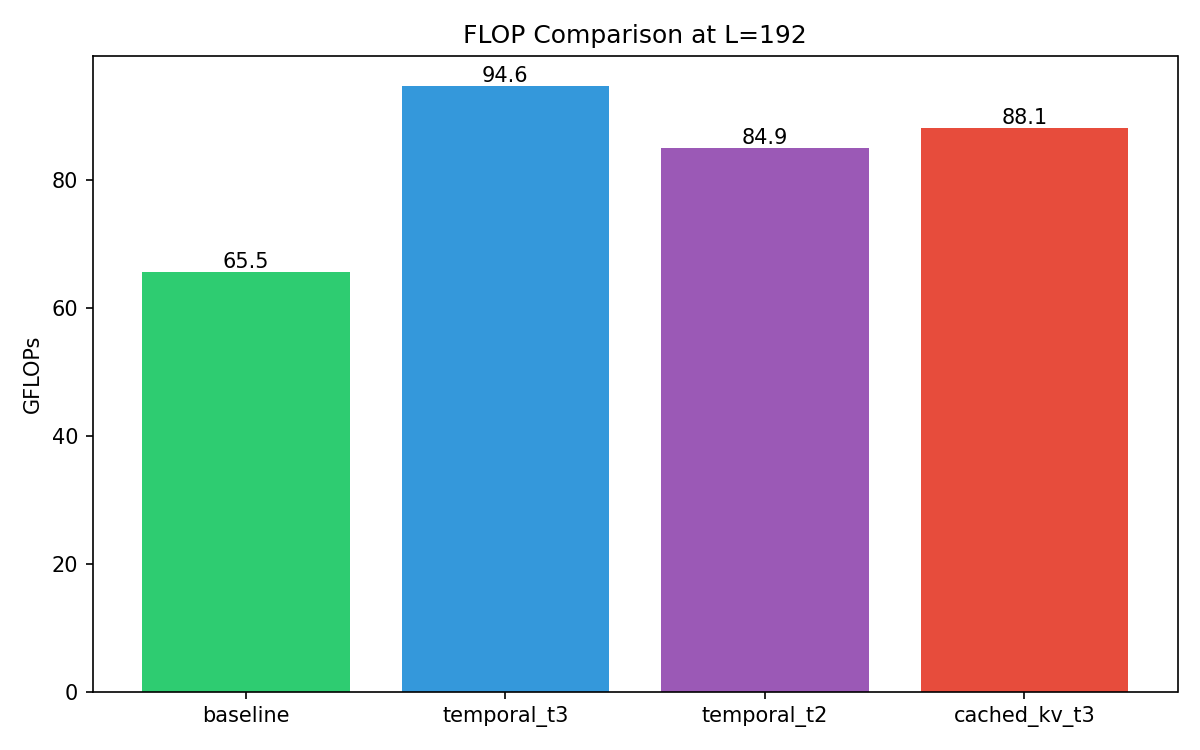
\includegraphics[width=0.9\columnwidth]{figures/fig1_flop_comparison.png}
    \caption{FLOP comparison across attention variants.}
    \label{fig:flop_comparison}
\end{figure}

\subsection{H-M2: Convergence --- FAIL}

\begin{table}[h]
\centering
\begin{tabular}{@{}lcc@{}}
\toprule
\textbf{Metric} & \textbf{Expected} & \textbf{Actual} \\
\midrule
Entropy Step 1 & Reference & 4.099 \\
Entropy Step 2 & $<$ 4.099 & 4.139 (+0.98\%) \\
\bottomrule
\end{tabular}
\caption{Convergence test results.}
\label{tab:convergence}
\end{table}

\textbf{Status:} \textbf{FAIL} --- Attention entropy \emph{increases} across steps.

\begin{figure}[t]
    \centering
    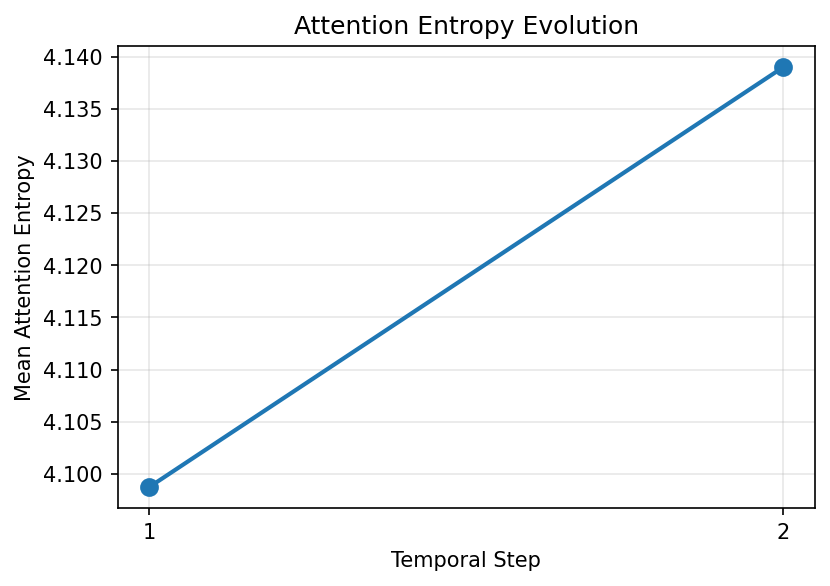
\includegraphics[width=0.9\columnwidth]{figures/entropy_curve.png}
    \caption{Attention entropy increases across temporal steps, contradicting convergence hypothesis.}
    \label{fig:entropy}
\end{figure}

\subsection{H-C1: Scaling --- FAIL}

\begin{table}[h]
\centering
\begin{tabular}{@{}lc@{}}
\toprule
\textbf{Seq Length} & \textbf{Reduction} \\
\midrule
128 & 5.31\% \\
512 & 5.31\% \\
1024 & 5.31\% \\
\bottomrule
\end{tabular}
\caption{FLOP reduction across sequence lengths.}
\label{tab:scaling}
\end{table}

\textbf{Status:} \textbf{FAIL} --- Constant reduction, no scaling advantage.

\begin{figure}[t]
    \centering
    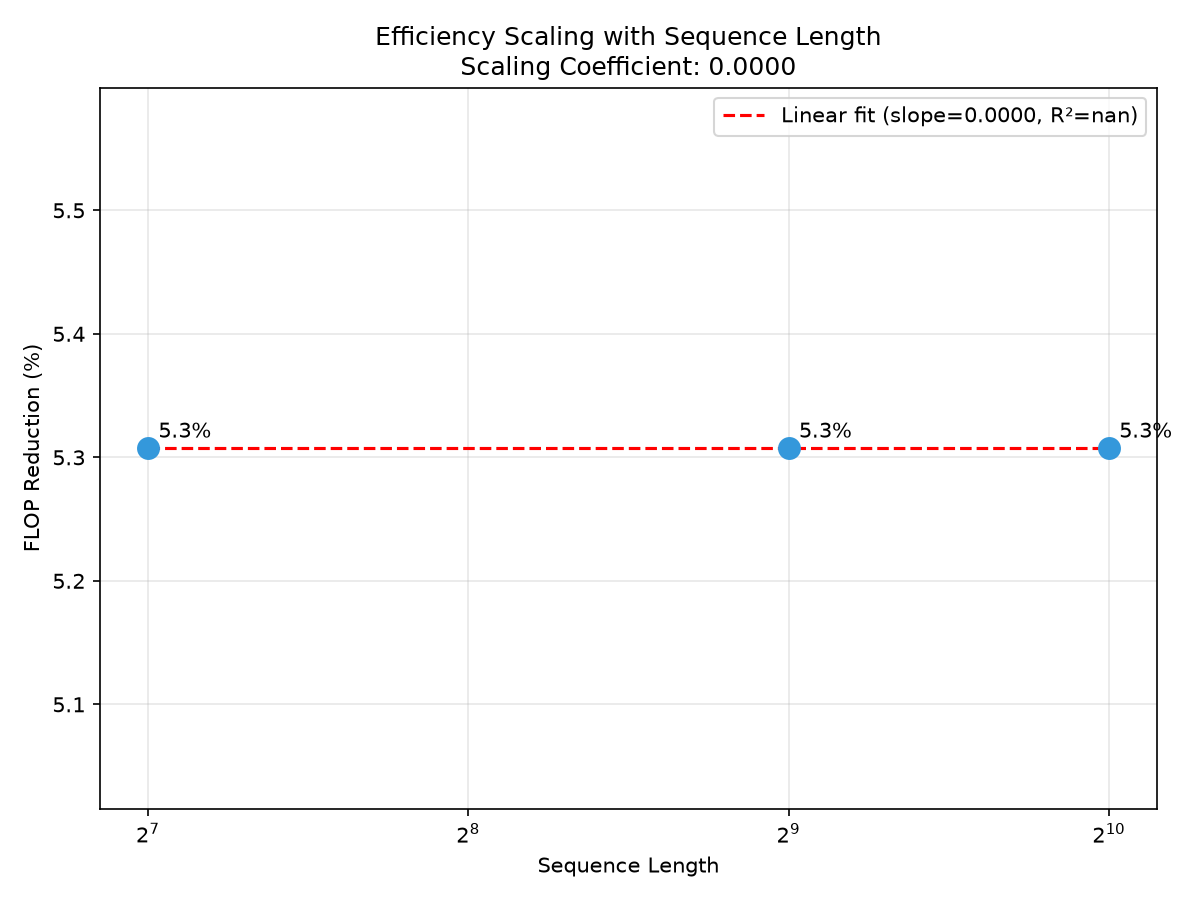
\includegraphics[width=0.9\columnwidth]{figures/fig2_scaling_curve.png}
    \caption{FLOP reduction is constant across sequence lengths.}
    \label{fig:scaling}
\end{figure}

\subsection{Summary}

\begin{table}[h]
\centering
\begin{tabular}{@{}llc@{}}
\toprule
\textbf{Sub-Hypothesis} & \textbf{Gate} & \textbf{Status} \\
\midrule
H-E1 Existence & MUST\_WORK & \textbf{PASS} \\
H-M1 Efficiency & MUST\_WORK & \textbf{PASS} \\
H-M2 Convergence & SHOULD\_WORK & \textbf{FAIL} \\
H-C1 Scaling & SHOULD\_WORK & \textbf{FAIL} \\
\bottomrule
\end{tabular}
\caption{Sub-hypothesis verification summary.}
\label{tab:summary}
\end{table}

\textbf{Core efficiency validated. Proposed mechanism falsified.}
